%%% Article Template
%%% Set Document layout
\documentclass[final, 12pt]{article}

%%%%%%%%%% Set Name, Subject, Date ...
\newcommand{\toppic}{Analysis}
\newcommand{\mytitle}{Analysis}
\newcommand{\workingDate}{12.01.2023}
\newcommand{\userName}{Jonathan Mayer}
%%
\usepackage{options}

%%%%%%%%%% Begin the document
\begin{document}  
\begin{center}
    {\textbf {\huge \mytitle}}\\[5mm]   % titel
    {\large \userName} \\[5mm]          % User Name
    \workingDate\\                      % Working Date
\end{center} %%%%%%%%%% Titel %%%%%%%%%%%%%%

%%
\section{Begriffe}
\begin{center}
    \begin{tblr}{ll}
        \textbf{Symbol}         & \textbf{Bedeutung} \\ \hline[1.5pt]
        $R$                    & Relation \\\hline
        $\in/ \notin$          & Element / kein Element von \\\hline
        $\forall / \nexists$   & für alle / für kein \\\hline
        $\exists$              & Existenzquantor, mindestens ein \\\hline
        $\exists !$            & Anzahlquantor, genau ein \\\hline
        $A \subset B$          & echte Teilmenge, $a \in A \land a,b \in B:\exists b\notin A$\\ \hline
        $A \subseteq B$             & Teilmenge $a \in A \land a,b \in B$ \\\hline
        $]1,3[$, $(1,3)$       & $1<x<3$ \\\hline
        $[1,3]$                & $1\leq x \leq 3$ \\\hline
        $\Rightarrow$          & genau dann wenn \\\hline
        $\Leftrightarrow$      & aus Aussage A folg B und umgekehrt \\\hline
        $\rightarrow$          & Abbildungsvorschrift für Mengen \\\hline
        $\mapsto$              & Abbildungsvorschrift für Elemente \\\hline
        $\circ$                & Komposition / Verkettung von Funktionen \\\hline
        $\land\ /\ \lor$       & und / oder \\\hline
        Lemma                  & Hilfssatz \\\hline
        $\overline{z}, \ z^*$  & konjungiert komplexe Zahl \\\hline
        $\preccurlyeq$         & beliebiges Symbol \\\hline
        $\stackrel{?}{=}$      & zu zeigen \\\hline
        $\stackrel{!}{=}$      & soll erfüllt sein um ... zu zeigen \\\hline
        $:=, \equiv$           & definiere \\\hline
        $\cup,\cap, /$         & Vereinigung, Durchschnitt, Subtrahiert \\\hline
        disjunkt               & $A \cap B = \{\}$ \\\hline
        infimum \\\hline
        supremum \\\hline
        notwendiges Kriterium & muss immer erfüllt sein, reicht aber nicht aus\\ \hline
        hinreichendes Kriterium & wenn erfüllt dann ... \\ \hline
        Nullfolge  &   $(a_k)_k$ ist eine Nullfolge wenn $\lim_{k\to\infty}a_k=0$\\ \hline
        surjektiv & $\forall y \in Y : \exists \  x \in X:f(x)=y$ \ref{subs:surjektivitaet}\\ \hline
        injektiv &$\forall x_1,x_2 \in X:f(x_1)=f(x_2) \Rightarrow x_1=x_2$   \ref{subs:injektivitaet}\\ \hline
        bijektiv & $\forall y \in Y : \exists ! \  x \in X:f(x)=y$\ref{subs:bijektivitaet}\\ \hline
        beschränkte Folge & $\exists b,c : \forall n: b<a_n<c$ \\ \hline
        nach oben beschränkte Folge &  $\exists b: \forall n: a_n<b$\\ \hline
        nach unten beschränkte Folge &  $\exists b: \forall n: b<a_n$\\ \hline
    \end{tblr}
\end{center}




\section{Relationen und Funktionen}

\subsection{Funktionen}
\subsubsection{surjektivität:}\label{subs:surjektivitaet}
wenn es für jedes $y$ aus $Y$ \textbf{mindestens} ein $x \in X$ mit $f(x) = y$ gibt.\\
wenn es auf jeder gedachten Horizontalen in der Zielmenge \textbf{mindestens} einen Schnittpunkt mit der Funktion gibt.\\
$\forall y \in Y : \exists \  x \in X:f(x)=y$

\subsubsection{injektivität}\label{subs:injektivitaet}
wenn es für jedes $y \in $ vom Wertebereich $Y$ \textbf{höchstens} ein $x \in$ der Definitionsmenge $X$ gibt.\\
Für jede gedachte Horizontale gibt es \textbf{höchstens} einen Schnittpunkt mit der Funktion.\\
$\forall x_1,x_2 \in X:f(x_1)=f(x_2) \Rightarrow x_1=x_2$\\
$\forall b \in B: \exists$ höchstens ein $a \in A :f(a)=b$\\

\subsubsection{bijektivität}\label{subs:bijektivitaet}  
\textbf{Injektiv und surjektiv}\\
wenn es für jedes $y\in Y$  \textbf{genau ein} $x \in X$ gibt.\\
wenn es auf jeder gedachten Horizontalen in der Zielmenge \textbf{genau einen Schnittpunkt} mit der Funktion gibt.\\
$\forall y \in Y : \exists ! \  x \in X:f(x)=y$\\

Bei stetigen Funktionen darf der Grenzwert und die Funktion vertauscht werten ($\lim\limits_{x\to 0 }e^{x\cdot \ln (x)}=e^{\lim\limits_{x\to 0 }x\cdot \ln(x)}$).

\section{Folgen}

\textbf{beschränkte Folge:} $(a_n)_n$ ist beschränkt wenn $\exists b,c : \forall n: b<a_n<c$.\\

\textbf{nach oben beschränkte Folge:} $(a_n)_n$ ist nach oben beschränkt wenn $\exists b: \forall n: a_n<b$.

\textbf{nach unten beschränkte Folge:} $(a_n)_n$ ist nach unten beschränkt wenn $\exists b: \forall n: b<a_n$.



\section{Reihen}
\begin{description}
    \item[\textbf{Definition:}] Eine Reihe ist eine Partialsumme einer Folge $(p_n)_n = \left(\sum\limits_{i=0}^{n}a_i \right)_n$, $p_n$... Reihe, $a_i$... Folge\\
    \item[\textbf{harmonische Reihe:}] $\sum\limits_{k=1}^{\infty}\frac{1}{k}$ ist divergent\\
    \item[$\sum\limits_{k=1}^{\infty}\frac{1}{k^r}$] konvergiert für $r\geq 2$\\
\end{description}




\subsection{Konvergenzkriterien}

\textbf{Definition Konvergenz:} \\

\textbf{Definition absolute Konvergenz:} \\$\sum\limits_{k=1}^{\infty}\frac{1}{k}$ 

\subsubsection{Minoranten- Majoranten Kriterium}

\subsection{Quotientenkriterium}

\subsection{Wurzelkriterium}

%%
\section{Stetigkeit}

\textbf{Definition Stetigkeit:}\\
$\forall \epsilon > 0 :\exists \delta > 0 : |x-a|<\delta : |f(x)-f(a)|<\epsilon$\\
$\forall \epsilon > 0 :\exists \delta > 0 : f(U_{\delta}(a) \subseteq U_{\epsilon}(f(a)))$\\
$\forall \epsilon > 0\  \exists \delta >0 : \text{sodass aus } |x-a|<\delta \text{ stets } |f(x)-f(a)|<\epsilon \text{ folgt}$\\

\textbf{Definition Unstetigkeit:} $\exists \epsilon > 0 \forall\  \delta > 0 :\exists x \in D : |x-x_0|< \delta \wedge |f(x)-f(x_0)|>\epsilon$

\subsection{links-rechtsseitiger Grenzwetz:}

$\lim\limits_{x\to x_0^-}f(x) = \lim\limits_{x\to x_0^+} f(x)$

$x_0$ wird von rechts und links angenähert. Sind beide Grenzwerte gleich ist die Funktion stetig.


\subsection{$\epsilon - \delta$ Kriterium}

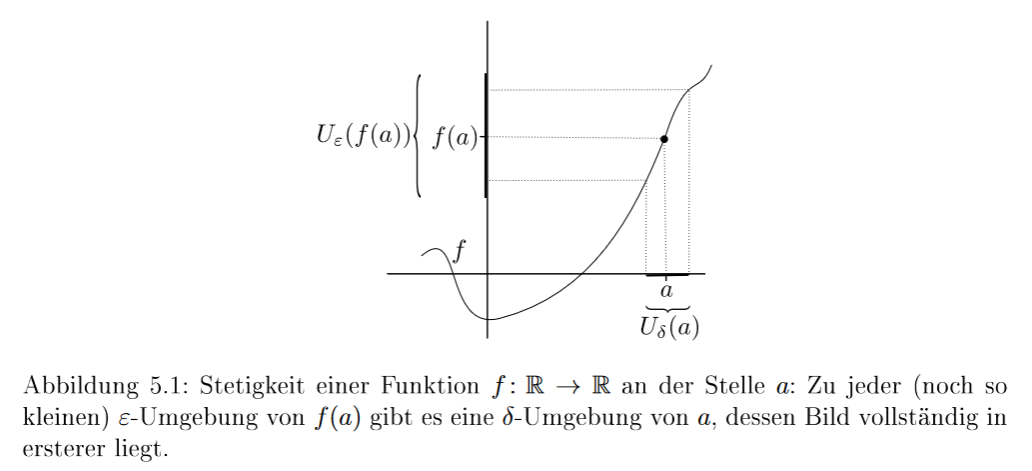
\includegraphics[width= \textwidth]{./pictures/Stetigkeit.png}
$\epsilon$ quer darf nach oben abgeschätz werden.
Zuerst delta ausrechnen
dann Beweis nochmal schön hinschrieben.\\

$|x-a|<\delta$\\
$|f(x)-f(a)|< \epsilon|$\\

$\epsilon$ darf gewählt werden

Nicht Stetigkeit beweisen:\\
>links und rechtsseitiger Grenzwert\\
>epsilon delta Kriterium

-->

$\exists \epsilon > 0 :\forall \delta >0 \exists x |x-x_0| < \delta \vee |f(x)-f(x_0) > \epsilon|$



\section{l´Hospital}

\captionsetup{type=figure}
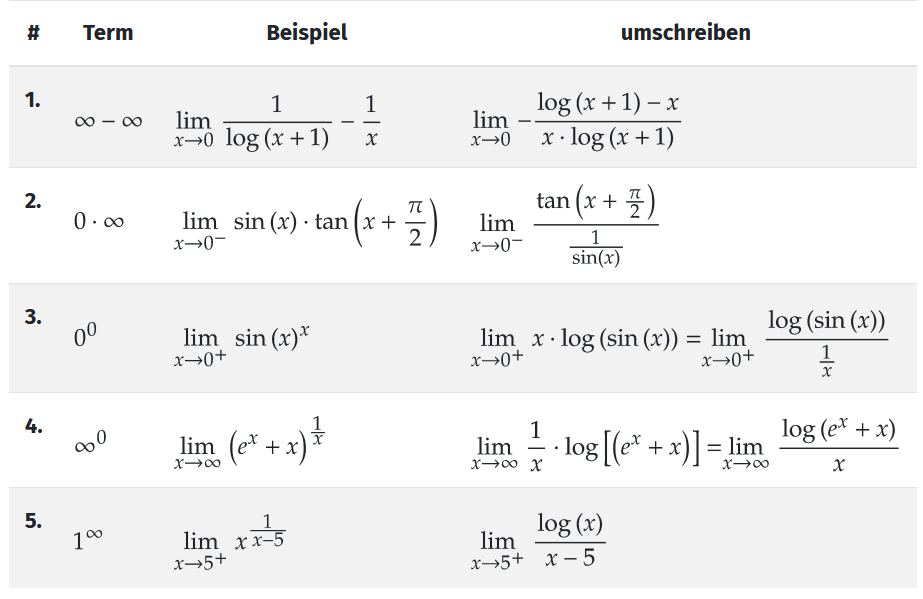
\includegraphics[width=.7\textwidth]{pictures/Umformung_l_Hospital.png}
\caption{Umformung für l´Hospital}\label{fig:Umf_l_Hospital}



%%% Verzeichnisse
\newpage
%\listoftables
%\listoffigures
%\printbibliography{}
%%%%%% Document end
\end{document}     %%% End the document


